% Options for packages loaded elsewhere
\PassOptionsToPackage{unicode}{hyperref}
\PassOptionsToPackage{hyphens}{url}
\PassOptionsToPackage{dvipsnames,svgnames,x11names}{xcolor}
%
\documentclass[
  11pt,
]{article}

\usepackage{amsmath,amssymb}
\usepackage{iftex}
\ifPDFTeX
  \usepackage[T1]{fontenc}
  \usepackage[utf8]{inputenc}
  \usepackage{textcomp} % provide euro and other symbols
\else % if luatex or xetex
  \usepackage{unicode-math}
  \defaultfontfeatures{Scale=MatchLowercase}
  \defaultfontfeatures[\rmfamily]{Ligatures=TeX,Scale=1}
\fi
\usepackage{lmodern}
\ifPDFTeX\else  
    % xetex/luatex font selection
\fi
% Use upquote if available, for straight quotes in verbatim environments
\IfFileExists{upquote.sty}{\usepackage{upquote}}{}
\IfFileExists{microtype.sty}{% use microtype if available
  \usepackage[]{microtype}
  \UseMicrotypeSet[protrusion]{basicmath} % disable protrusion for tt fonts
}{}
\makeatletter
\@ifundefined{KOMAClassName}{% if non-KOMA class
  \IfFileExists{parskip.sty}{%
    \usepackage{parskip}
  }{% else
    \setlength{\parindent}{0pt}
    \setlength{\parskip}{6pt plus 2pt minus 1pt}}
}{% if KOMA class
  \KOMAoptions{parskip=half}}
\makeatother
\usepackage{xcolor}
\usepackage[margin=1in]{geometry}
\setlength{\emergencystretch}{3em} % prevent overfull lines
\setcounter{secnumdepth}{-\maxdimen} % remove section numbering
% Make \paragraph and \subparagraph free-standing
\ifx\paragraph\undefined\else
  \let\oldparagraph\paragraph
  \renewcommand{\paragraph}[1]{\oldparagraph{#1}\mbox{}}
\fi
\ifx\subparagraph\undefined\else
  \let\oldsubparagraph\subparagraph
  \renewcommand{\subparagraph}[1]{\oldsubparagraph{#1}\mbox{}}
\fi


\providecommand{\tightlist}{%
  \setlength{\itemsep}{0pt}\setlength{\parskip}{0pt}}\usepackage{longtable,booktabs,array}
\usepackage{calc} % for calculating minipage widths
% Correct order of tables after \paragraph or \subparagraph
\usepackage{etoolbox}
\makeatletter
\patchcmd\longtable{\par}{\if@noskipsec\mbox{}\fi\par}{}{}
\makeatother
% Allow footnotes in longtable head/foot
\IfFileExists{footnotehyper.sty}{\usepackage{footnotehyper}}{\usepackage{footnote}}
\makesavenoteenv{longtable}
\usepackage{graphicx}
\makeatletter
\def\maxwidth{\ifdim\Gin@nat@width>\linewidth\linewidth\else\Gin@nat@width\fi}
\def\maxheight{\ifdim\Gin@nat@height>\textheight\textheight\else\Gin@nat@height\fi}
\makeatother
% Scale images if necessary, so that they will not overflow the page
% margins by default, and it is still possible to overwrite the defaults
% using explicit options in \includegraphics[width, height, ...]{}
\setkeys{Gin}{width=\maxwidth,height=\maxheight,keepaspectratio}
% Set default figure placement to htbp
\makeatletter
\def\fps@figure{htbp}
\makeatother

\usepackage{graphicx}
\usepackage{array}
\usepackage{longtable}
\usepackage{booktabs}
\setlength{\extrarowheight}{4pt}
\renewcommand{\arraystretch}{1.5}
\newcolumntype{L}[1]{>{\raggedright\arraybackslash}p{#1}}
\newcolumntype{C}[1]{>{\centering\arraybackslash}p{#1}}
\newcolumntype{R}[1]{>{\raggedleft\arraybackslash}p{#1}}
\makeatletter
\makeatother
\makeatletter
\makeatother
\makeatletter
\@ifpackageloaded{caption}{}{\usepackage{caption}}
\AtBeginDocument{%
\ifdefined\contentsname
  \renewcommand*\contentsname{Table of contents}
\else
  \newcommand\contentsname{Table of contents}
\fi
\ifdefined\listfigurename
  \renewcommand*\listfigurename{List of Figures}
\else
  \newcommand\listfigurename{List of Figures}
\fi
\ifdefined\listtablename
  \renewcommand*\listtablename{List of Tables}
\else
  \newcommand\listtablename{List of Tables}
\fi
\ifdefined\figurename
  \renewcommand*\figurename{Figure}
\else
  \newcommand\figurename{Figure}
\fi
\ifdefined\tablename
  \renewcommand*\tablename{Table}
\else
  \newcommand\tablename{Table}
\fi
}
\@ifpackageloaded{float}{}{\usepackage{float}}
\floatstyle{ruled}
\@ifundefined{c@chapter}{\newfloat{codelisting}{h}{lop}}{\newfloat{codelisting}{h}{lop}[chapter]}
\floatname{codelisting}{Listing}
\newcommand*\listoflistings{\listof{codelisting}{List of Listings}}
\makeatother
\makeatletter
\@ifpackageloaded{caption}{}{\usepackage{caption}}
\@ifpackageloaded{subcaption}{}{\usepackage{subcaption}}
\makeatother
\makeatletter
\@ifpackageloaded{tcolorbox}{}{\usepackage[skins,breakable]{tcolorbox}}
\makeatother
\makeatletter
\@ifundefined{shadecolor}{\definecolor{shadecolor}{rgb}{.97, .97, .97}}
\makeatother
\makeatletter
\makeatother
\makeatletter
\makeatother
\ifLuaTeX
  \usepackage{selnolig}  % disable illegal ligatures
\fi
\IfFileExists{bookmark.sty}{\usepackage{bookmark}}{\usepackage{hyperref}}
\IfFileExists{xurl.sty}{\usepackage{xurl}}{} % add URL line breaks if available
\urlstyle{same} % disable monospaced font for URLs
\hypersetup{
  pdftitle={VIDEO FOOTAGE LICENSING AGREEMENT},
  colorlinks=true,
  linkcolor={blue},
  filecolor={Maroon},
  citecolor={Blue},
  urlcolor={Blue},
  pdfcreator={LaTeX via pandoc}}

\title{VIDEO FOOTAGE LICENSING AGREEMENT}
\author{}
\date{2025-11-13}

\begin{document}
\maketitle
\ifdefined\Shaded\renewenvironment{Shaded}{\begin{tcolorbox}[interior hidden, boxrule=0pt, borderline west={3pt}{0pt}{shadecolor}, sharp corners, enhanced, breakable, frame hidden]}{\end{tcolorbox}}\fi

\hypertarget{agreement}{%
\section{AGREEMENT}\label{agreement}}

This Video Footage Licensing Agreement (``Agreement'') is entered into
on \underline{\hspace{3cm}} (``Effective Date'') between:

\textbf{LICENSOR:}

\begin{table}[h]
\centering
\begin{tabular}{L{3.5cm}L{10.5cm}}
\toprule
\textbf{Field} & \textbf{Value} \\
\midrule
Company Name & Fifth Avenue Studios \\
Contact Name & Gil Raitses \\
Address & 1724 5th Ave, Bay Shore, NY 11706 \\
Phone & (212) 365-0255 \\
Email & gilraitses@gmail.com \\
\bottomrule
\end{tabular}
\end{table}

\textbf{LICENSEE:}

\emph{Please fill in the licensee information:}

\begin{table}[h]
\centering
\begin{tabular}{L{3.5cm}L{10.5cm}}
\toprule
\textbf{Field} & \textbf{Value} \\
\midrule
Company Name & \underline{\hspace{8cm}} \\
Address & \underline{\hspace{8cm}} \\
Contact Name & \underline{\hspace{8cm}} \\
Phone & \underline{\hspace{8cm}} \\
Email & \underline{\hspace{8cm}} \\
\bottomrule
\end{tabular}
\end{table}

\hypertarget{grant-of-license}{%
\section{1. GRANT OF LICENSE}\label{grant-of-license}}

\hypertarget{licensed-material}{%
\subsection{1.1 Licensed Material}\label{licensed-material}}

Licensor hereby grants to Licensee a non-exclusive license to use the
following video footage (``Licensed Material''):

\begin{table}[h]
\centering
\begin{tabular}{L{3.5cm}L{10.5cm}}
\toprule
\textbf{Property} & \textbf{Value} \\
\midrule
File Name & IMG\_3788.mov \\
Description & Video footage of Flaco the owl's first landing on Fifth Avenue on the night he was freed from the Central Park Zoo \\
Shot By & Eitan Raitses \\
Shot Date & February 4, 2024 \\
Shot Time & 11:27 PM \\
Duration & 15.83 seconds \\
Resolution & 720 × 1280 pixels (Full HD 1080p) \\
Frame Rate & 30.00 fps \\
File Size & 4.76 MB \\
\bottomrule
\end{tabular}
\end{table}

\hypertarget{rights-granted}{%
\subsection{1.2 Rights Granted}\label{rights-granted}}

Subject to the terms and conditions of this Agreement, Licensor grants
Licensee the following rights:

\begin{table}[h]
\centering
\begin{tabular}{L{3.5cm}L{10.5cm}}
\toprule
\textbf{Right} & \textbf{Description} \\
\midrule
Usage & Worldwide, perpetual use in documentary film production \\
Editing & Licensee may edit, modify, and enhance the Licensed Material as necessary for production purposes, including stabilization, sharpening, and color correction \\
\bottomrule
\end{tabular}
\end{table}

\textbf{Media Platforms:}

\begin{table}[h]
\centering
\begin{tabular}{L{5cm}C{3cm}}
\toprule
\textbf{Platform} & \textbf{Included} \\
\midrule
Theatrical release & Yes \\
Television broadcast & Yes \\
Streaming platforms & Yes \\
Digital distribution & Yes \\
Home video/DVD/Blu-ray & Yes \\
Promotional materials & Yes \\
Educational distribution & Yes \\
\bottomrule
\end{tabular}
\end{table}

\textbf{Multiple Uses:}

\begin{table}[h]
\centering
\begin{tabular}{L{5cm}C{3cm}}
\toprule
\textbf{Use Case} & \textbf{Included} \\
\midrule
Opening sequences & Yes \\
Transitional moments & Yes \\
Key narrative scenes & Yes \\
Closing sequences & Yes \\
\bottomrule
\end{tabular}
\end{table}

\hypertarget{restrictions}{%
\subsection{1.3 Restrictions}\label{restrictions}}

The following restrictions apply:

\begin{table}[h]
\centering
\begin{tabular}{L{3.5cm}L{10.5cm}}
\toprule
\textbf{Restriction} & \textbf{Description} \\
\midrule
Sublicensing & Licensee may not sublicense the Licensed Material without prior written consent \\
Defamatory Use & Licensee may not use the Licensed Material in a manner that is defamatory, libelous, or violates any third-party rights \\
Ownership Claims & Licensee may not claim ownership of the Licensed Material \\
Scope Limitation & Licensee may not use the Licensed Material for purposes other than the documentary production without additional licensing \\
\bottomrule
\end{tabular}
\end{table}

\hypertarget{compensation}{%
\section{2. COMPENSATION}\label{compensation}}

\hypertarget{license-fee}{%
\subsection{2.1 License Fee}\label{license-fee}}

In consideration for the rights granted herein, Licensee agrees to pay
Licensor a total license fee of:

\textbf{\$2,500.00} (Two Thousand Five Hundred Dollars)

This fee is based on the following valuation factors:

\begin{table}[h]
\centering
\begin{tabular}{L{5cm}L{2.5cm}L{6.5cm}}
\toprule
\textbf{Factor} & \textbf{Multiplier} & \textbf{Value} \\
\midrule
Base Rate (per usable second) & 1.00× & \$50.00 \\
Quality Multiplier & 0.50× & \\
Resolution Multiplier & 1.00× & \\
Content Significance Multiplier & 1.50× & \\
Narrative Significance Multiplier & 2.50× & \\
Multiple-Use Multiplier & 1.50× & \\
\textbf{Final Rate per Second} & & \textbf{\$140.62} \\
Total Usable Seconds & & 15.83 \\
\textbf{Calculated Value} & & \textbf{\$2,226} \\
\textbf{Premium Value} & & \textbf{\$2,713} \\
\bottomrule
\end{tabular}
\end{table}

\hypertarget{payment-terms}{%
\subsection{2.2 Payment Terms}\label{payment-terms}}

\emph{Please fill in the following payment terms:}

\begin{table}[h]
\centering
\begin{tabular}{L{3.5cm}L{10.5cm}}
\toprule
\textbf{Term} & \textbf{Value} \\
\midrule
Payment Deadline & Payment shall be made in full within \underline{\hspace{2cm}} days of the Effective Date \\
\vspace{0.3cm} & \\
Payment Method & Payment shall be made via: \underline{\hspace{6cm}} \\
\vspace{0.3cm} & \\
Payment Address & Payment shall be sent to: \underline{\hspace{6cm}} \\
\bottomrule
\end{tabular}
\end{table}

\hypertarget{late-payment}{%
\subsection{2.3 Late Payment}\label{late-payment}}

If payment is not received within the specified timeframe, Licensee
shall be liable for interest charges of 1.5\% per month on the
outstanding balance.

\hypertarget{delivery-of-materials}{%
\section{3. DELIVERY OF MATERIALS}\label{delivery-of-materials}}

\hypertarget{delivery}{%
\subsection{3.1 Delivery}\label{delivery}}

\emph{Please fill in the delivery method and deadline:}

Licensor shall deliver the Licensed Material to Licensee in the
following format:

\begin{table}[h]
\centering
\begin{tabular}{L{3.5cm}L{10.5cm}}
\toprule
\textbf{Requirement} & \textbf{Value} \\
\midrule
File Type & Original unedited source file (without watermarks) \\
Format & MOV file (IMG\_3788.mov) \\
\vspace{0.3cm} & \\
Delivery Method & \underline{\hspace{6cm}} (e.g., WeTransfer, Dropbox, etc.) \\
\vspace{0.3cm} & \\
Delivery Deadline & \underline{\hspace{2cm}} days from Effective Date \\
\bottomrule
\end{tabular}
\end{table}

\hypertarget{quality}{%
\subsection{3.2 Quality}\label{quality}}

Licensor warrants that the Licensed Material is the original, unedited
source file as captured. Licensee acknowledges that the Licensed
Material may require post-processing (stabilization, sharpening, color
correction) for optimal production use.

\hypertarget{warranties-and-representations}{%
\section{4. WARRANTIES AND
REPRESENTATIONS}\label{warranties-and-representations}}

\hypertarget{licensor-warranties}{%
\subsection{4.1 Licensor Warranties}\label{licensor-warranties}}

Licensor represents and warrants that:

\begin{table}[h]
\centering
\begin{tabular}{L{3.5cm}L{10.5cm}}
\toprule
\textbf{Warranty} & \textbf{Description} \\
\midrule
Ownership & Licensor is the sole owner of the Licensed Material or has the right to grant the license herein \\
Intellectual Property & The Licensed Material does not infringe upon any copyright, trademark, or other intellectual property rights \\
Privacy Rights & The Licensed Material does not violate any privacy rights or publicity rights of any person \\
Authority & Licensor has the full right and authority to enter into this Agreement \\
\bottomrule
\end{tabular}
\end{table}

\hypertarget{licensee-warranties}{%
\subsection{4.2 Licensee Warranties}\label{licensee-warranties}}

Licensee represents and warrants that:

\begin{table}[h]
\centering
\begin{tabular}{L{3.5cm}L{10.5cm}}
\toprule
\textbf{Warranty} & \textbf{Description} \\
\midrule
Usage Compliance & Licensee will use the Licensed Material only in accordance with this Agreement \\
Lawful Use & Licensee will not use the Licensed Material in any defamatory or unlawful manner \\
Authority & Licensee has the full right and authority to enter into this Agreement \\
\bottomrule
\end{tabular}
\end{table}

\hypertarget{credit-and-attribution}{%
\section{5. CREDIT AND ATTRIBUTION}\label{credit-and-attribution}}

\hypertarget{credit-requirement}{%
\subsection{5.1 Credit Requirement}\label{credit-requirement}}

Licensee agrees to provide credit in the documentary's credits and
promotional materials in the following format:

\textit{"Flaco Footage Courtesy of Eitan Raitses / Fifth Avenue Studios"}

or

\textit{"Additional Footage: Eitan Raitses (Cinematographer) and Gil Raitses / Fifth Avenue Studios"}

\emph{Note: Eitan Raitses filmed the footage. Gil Raitses is the owner
of Fifth Avenue Studios, which owns the footage.}

\hypertarget{credit-placement}{%
\subsection{5.2 Credit Placement}\label{credit-placement}}

Credit shall appear:

\begin{table}[h]
\centering
\begin{tabular}{L{3.5cm}L{10.5cm}}
\toprule
\textbf{Location} & \textbf{Requirement} \\
\midrule
End Credits & In the end credits of the documentary \\
Promotional Materials & In all promotional materials where other footage credits appear \\
Size and Position & In a size and position comparable to other similar credits \\
\bottomrule
\end{tabular}
\end{table}

\hypertarget{indemnification}{%
\section{6. INDEMNIFICATION}\label{indemnification}}

\hypertarget{licensor-indemnification}{%
\subsection{6.1 Licensor
Indemnification}\label{licensor-indemnification}}

Licensor agrees to indemnify, defend, and hold harmless Licensee from
any claims, damages, losses, or expenses (including reasonable
attorney's fees) arising from:

\begin{table}[h]
\centering
\begin{tabular}{L{3.5cm}L{10.5cm}}
\toprule
\textbf{Source} & \textbf{Description} \\
\midrule
Warranty Breach & Breach of Licensor's warranties \\
Infringement Claims & Claims that the Licensed Material infringes any third-party rights \\
Agreement Breach & Claims arising from Licensor's breach of this Agreement \\
\bottomrule
\end{tabular}
\end{table}

\hypertarget{licensee-indemnification}{%
\subsection{6.2 Licensee
Indemnification}\label{licensee-indemnification}}

Licensee agrees to indemnify, defend, and hold harmless Licensor from
any claims, damages, losses, or expenses (including reasonable
attorney's fees) arising from:

\begin{table}[h]
\centering
\begin{tabular}{L{3.5cm}L{10.5cm}}
\toprule
\textbf{Source} & \textbf{Description} \\
\midrule
Scope Violation & Licensee's use of the Licensed Material beyond the scope of this Agreement \\
Agreement Breach & Claims arising from Licensee's breach of this Agreement \\
Combined Use & Claims arising from Licensee's use of the Licensed Material in combination with other materials \\
\bottomrule
\end{tabular}
\end{table}

\hypertarget{term-and-termination}{%
\section{7. TERM AND TERMINATION}\label{term-and-termination}}

\hypertarget{term}{%
\subsection{7.1 Term}\label{term}}

This Agreement shall commence on the Effective Date and shall continue
in perpetuity, unless terminated earlier in accordance with this
Section.

\hypertarget{termination-for-breach}{%
\subsection{7.2 Termination for Breach}\label{termination-for-breach}}

Either party may terminate this Agreement immediately upon written
notice if the other party materially breaches this Agreement and fails
to cure such breach within thirty (30) days after written notice.

\hypertarget{effect-of-termination}{%
\subsection{7.3 Effect of Termination}\label{effect-of-termination}}

Upon termination:

\begin{table}[h]
\centering
\begin{tabular}{L{3.5cm}L{10.5cm}}
\toprule
\textbf{Effect} & \textbf{Description} \\
\midrule
Cessation of Use & Licensee shall cease all use of the Licensed Material \\
Completed Productions & Licensee shall have no obligation to remove the Licensed Material from completed productions already distributed \\
Payments & All payments made prior to termination shall be non-refundable \\
\bottomrule
\end{tabular}
\end{table}

\hypertarget{miscellaneous}{%
\section{8. MISCELLANEOUS}\label{miscellaneous}}

\hypertarget{entire-agreement}{%
\subsection{8.1 Entire Agreement}\label{entire-agreement}}

This Agreement constitutes the entire agreement between the parties and
supersedes all prior negotiations, representations, or agreements
relating to the subject matter herein.

\hypertarget{modification}{%
\subsection{8.2 Modification}\label{modification}}

This Agreement may only be modified by written agreement signed by both
parties.

\hypertarget{governing-law}{%
\subsection{8.3 Governing Law}\label{governing-law}}

This Agreement shall be governed by and construed in accordance with the
laws of the State of New York, without regard to its conflict of law
provisions.

\hypertarget{dispute-resolution}{%
\subsection{8.4 Dispute Resolution}\label{dispute-resolution}}

Any disputes arising under this Agreement shall be resolved through:

\emph{Please fill in arbitration organization if needed:}

\begin{table}[h]
\centering
\begin{tabular}{C{1cm}L{13cm}}
\toprule
\textbf{Step} & \textbf{Process} \\
\midrule
1 & Good faith negotiation between the parties \\
2 & If negotiation fails, through mediation \\
3 & If mediation fails, through binding arbitration in accordance with the rules of \underline{\hspace{4cm}} \\
\bottomrule
\end{tabular}
\end{table}

\hypertarget{severability}{%
\subsection{8.5 Severability}\label{severability}}

If any provision of this Agreement is found to be invalid or
unenforceable, the remaining provisions shall remain in full force and
effect.

\hypertarget{assignment}{%
\subsection{8.6 Assignment}\label{assignment}}

This Agreement may not be assigned by either party without the prior
written consent of the other party, except that Licensee may assign this
Agreement to an affiliate or successor in connection with a merger or
acquisition.

\hypertarget{notices}{%
\subsection{8.7 Notices}\label{notices}}

All notices required under this Agreement shall be in writing and
delivered to the addresses specified above, or to such other addresses
as may be designated in writing by either party.

\hypertarget{force-majeure}{%
\subsection{8.8 Force Majeure}\label{force-majeure}}

Neither party shall be liable for any failure or delay in performance
due to circumstances beyond its reasonable control, including but not
limited to acts of God, war, terrorism, or natural disasters.

\hypertarget{signatures}{%
\section{9. SIGNATURES}\label{signatures}}

IN WITNESS WHEREOF, the parties have executed this Agreement as of the
Effective Date.

\vspace{1cm}

\begin{table}[h]
\centering
\begin{tabular}{p{0.45\textwidth}p{0.45\textwidth}}
\hline
\textbf{LICENSOR} & \textbf{LICENSEE} \\
\hline
\vspace{2cm} & \vspace{2cm} \\
Fifth Avenue Studios & \underline{\hspace{5cm}} \\
\hline
\vspace{1cm} & \vspace{1cm} \\
\underline{\hspace{5cm}} & \underline{\hspace{5cm}} \\
Signature & Signature \\
\hline
\vspace{0.5cm} & \vspace{0.5cm} \\
Gil Raitses & \underline{\hspace{5cm}} \\
Print Name & Print Name \\
\hline
\vspace{0.5cm} & \vspace{0.5cm} \\
\underline{\hspace{5cm}} & \underline{\hspace{5cm}} \\
Title & Title \\
\hline
\vspace{0.5cm} & \vspace{0.5cm} \\
\underline{\hspace{5cm}} & \underline{\hspace{5cm}} \\
Date & Date \\
\hline
\end{tabular}
\end{table}

\newpage

\hypertarget{appendix-a-technical-specifications}{%
\section{APPENDIX A: TECHNICAL
SPECIFICATIONS}\label{appendix-a-technical-specifications}}

\hypertarget{video-footage-details}{%
\subsection{Video Footage Details}\label{video-footage-details}}

\begin{table}[h]
\centering
\begin{tabular}{L{4.5cm}L{9.5cm}}
\toprule
\textbf{Property} & \textbf{Value} \\
\midrule
File Name & IMG\_3788.mov \\
Shot By & Eitan Raitses \\
Shot Date & February 4, 2024 \\
Shot Time & 11:27 PM \\
Duration & 15.83 seconds \\
Resolution & 720 × 1280 pixels \\
Resolution Category & Full HD (1080p) \\
Frame Rate & 30.00 fps \\
Total Frames & 475 frames \\
File Size & 4.76 MB \\
Color Depth & 8-bit \\
Codec & Unknown \\
\bottomrule
\end{tabular}
\end{table}

\hypertarget{quality-metrics}{%
\subsection{Quality Metrics}\label{quality-metrics}}

\begin{table}[h]
\centering
\begin{tabular}{L{4.5cm}L{9.5cm}}
\toprule
\textbf{Metric} & \textbf{Value} \\
\midrule
Sharpness Score & 33.65 \\
Brightness & 72.8/255 \\
Contrast & 44.53 \\
Noise Level & 5.32 (Very Clean) \\
Exposure Score & 98.0/100 \\
Stability Score & 5.43 \\
Smoothness Score & 0.937 \\
Color Compression Score & 0.876 \\
Overall Quality Score & 49.7/100 \\
\bottomrule
\end{tabular}
\end{table}

\hypertarget{content-analysis}{%
\subsection{Content Analysis}\label{content-analysis}}

\begin{table}[h]
\centering
\begin{tabular}{L{4.5cm}L{9.5cm}}
\toprule
\textbf{Metric} & \textbf{Value} \\
\midrule
Frames Analyzed & 32 frames \\
Frames with Subject (Bird/Owl) & 14 frames (43.8\%) \\
Subject Visible Throughout & No \\
Rare/Unique Event & Yes \\
Narrative Significance Score & 100/100 (high importance) \\
Story Importance & High importance \\
Multiple-Use Potential & Yes \\
\bottomrule
\end{tabular}
\end{table}

\hypertarget{usability-analysis}{%
\subsection{Usability Analysis}\label{usability-analysis}}

\begin{table}[h]
\centering
\begin{tabular}{L{4.5cm}C{3cm}C{3cm}}
\toprule
\textbf{Category} & \textbf{Seconds} & \textbf{Percentage} \\
\midrule
Total Duration & 15.83 & 100.0\% \\
Usable Seconds & 15.83 & 100.0\% \\
High Quality Seconds & 6.93 & 43.8\% \\
Usable Segments & 1 & -- \\
\bottomrule
\end{tabular}
\end{table}

\hypertarget{appendix-b-valuation-breakdown}{%
\section{APPENDIX B: VALUATION
BREAKDOWN}\label{appendix-b-valuation-breakdown}}

\hypertarget{rate-calculation}{%
\subsection{Rate Calculation}\label{rate-calculation}}

\begin{figure}[h]
\centering
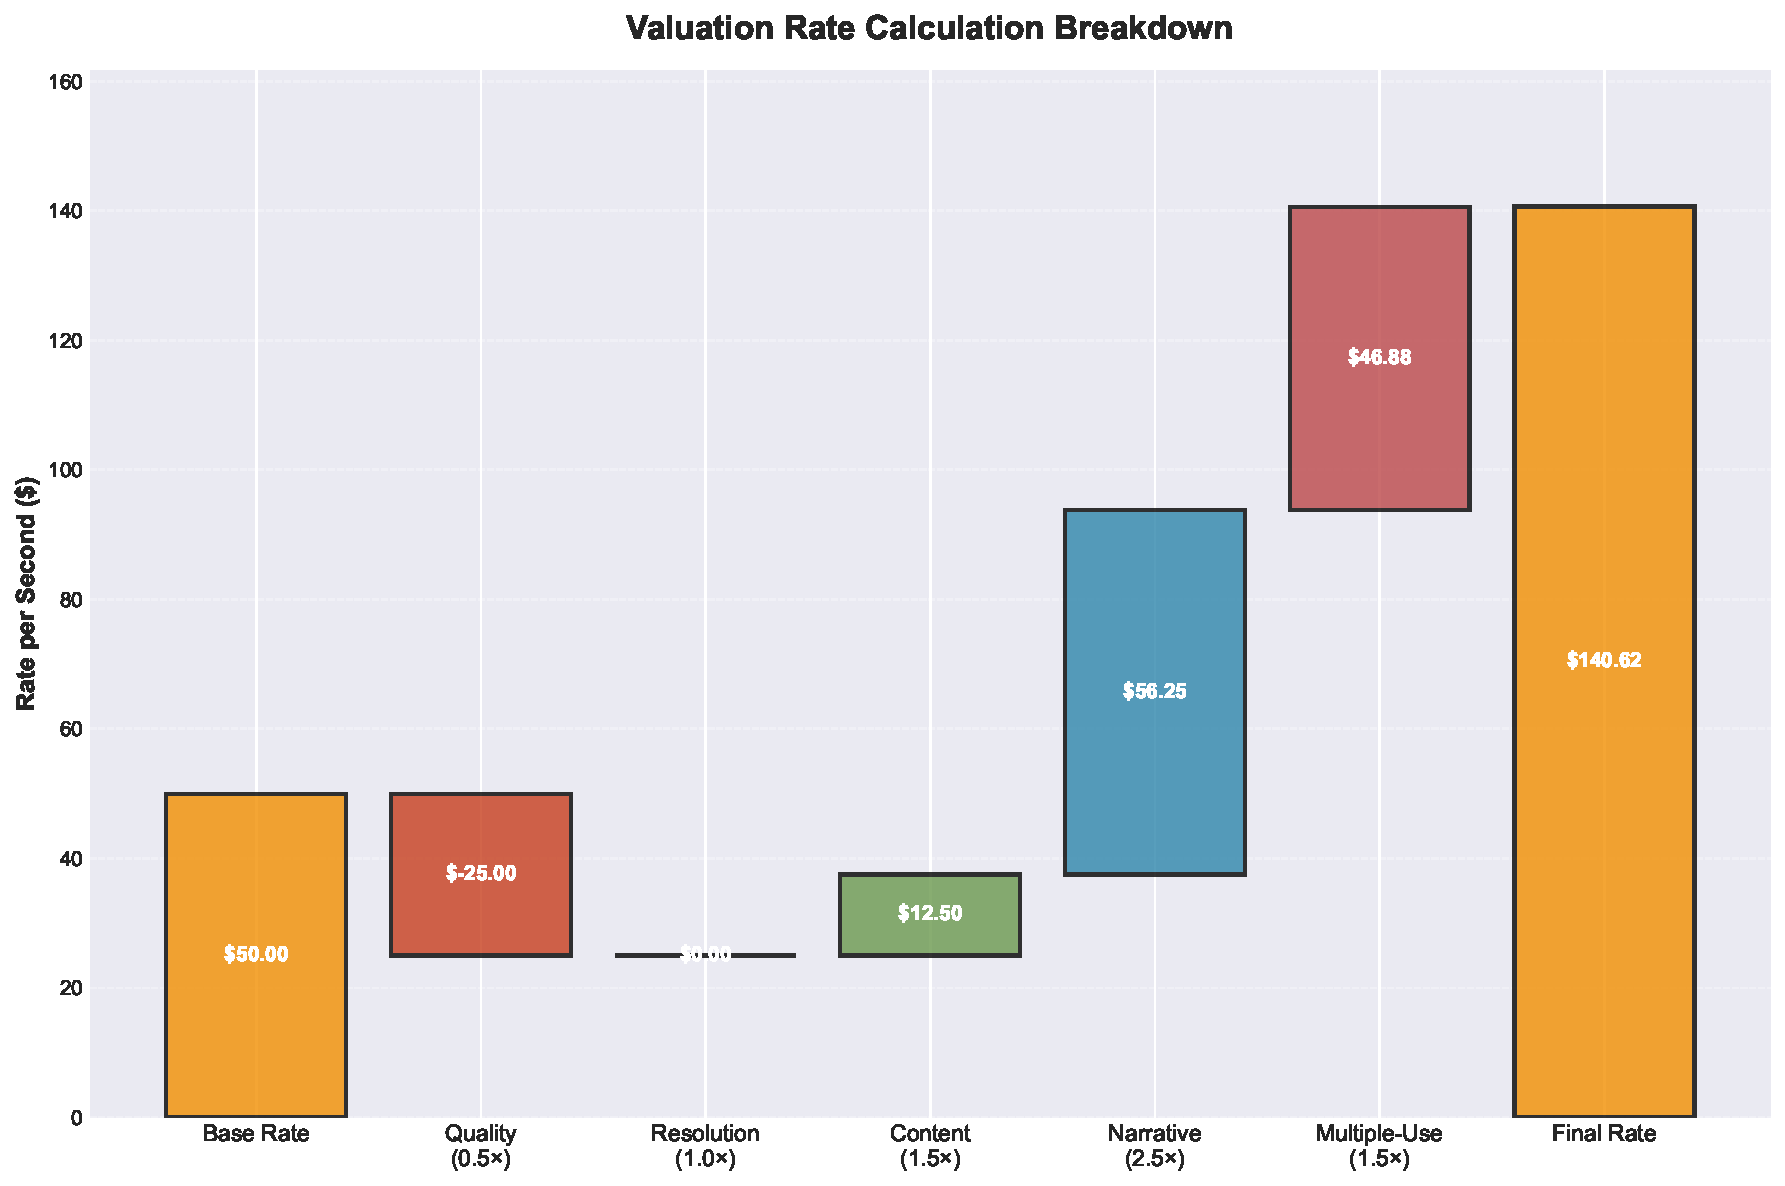
\includegraphics[width=0.9\textwidth]{figures/valuation_breakdown.pdf}
\caption{Valuation Rate Calculation Breakdown - Step-by-step waterfall chart showing how base rate (\$50/second) is modified by quality (0.5×), resolution (1.0×), content significance (1.5×), narrative significance (2.5×), and multiple-use (1.5×) multipliers to arrive at final rate of \$140.62 per usable second. Each bar segment represents the incremental value added by each factor.}
\label{fig-valuation-breakdown-agreement}
\end{figure}

\begin{figure}[h]
\centering
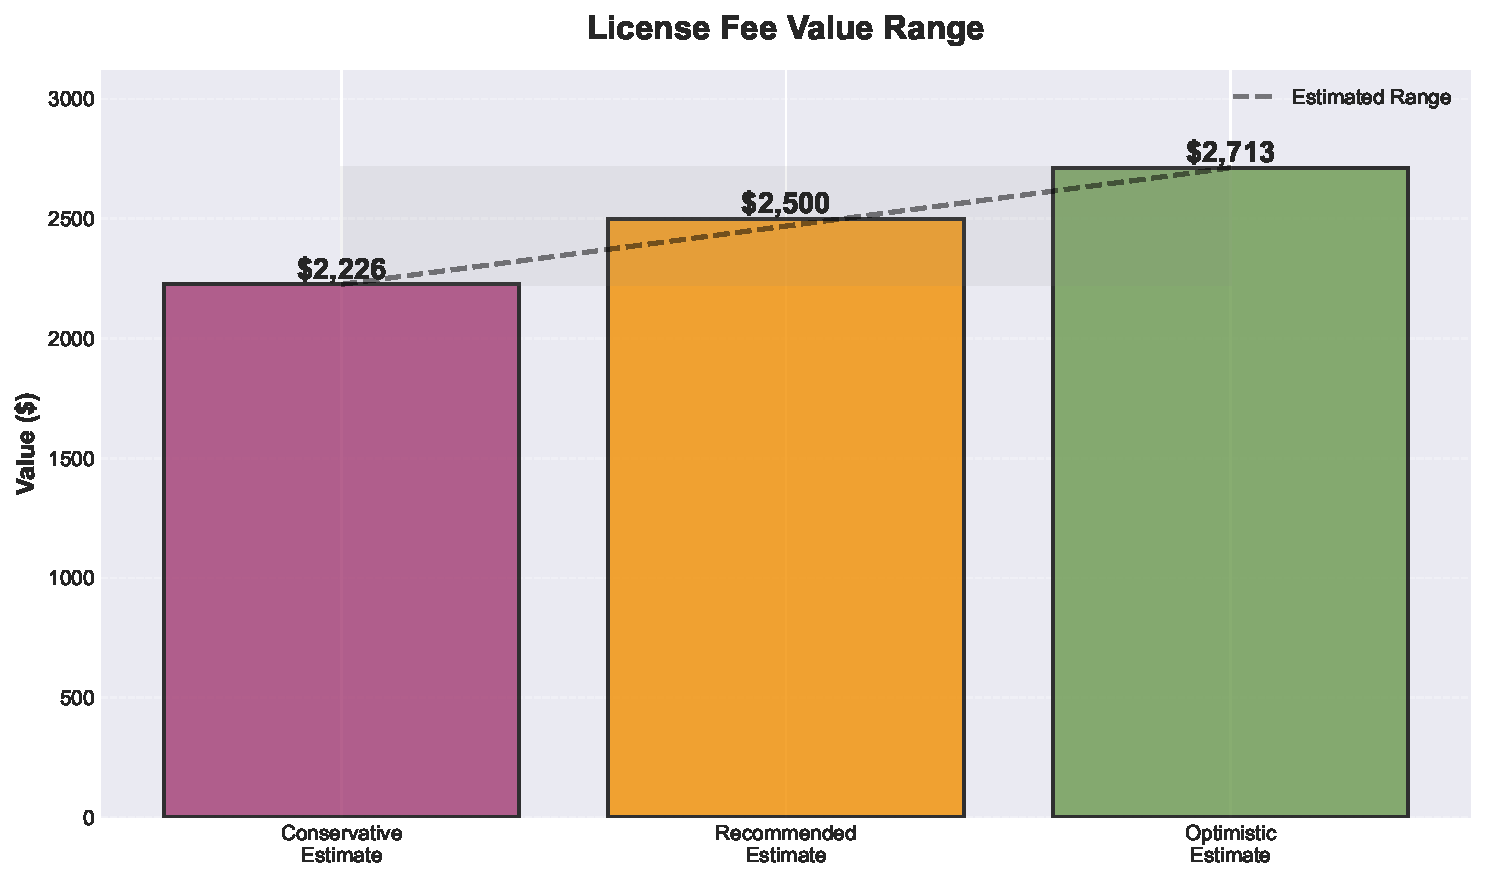
\includegraphics[width=0.85\textwidth]{figures/value_range.pdf}
\caption{License Fee Value Range Comparison - Bar chart comparing conservative estimate (\$2,226), agreed license fee (\$2,500), and optimistic estimate (\$2,713). The gray shaded area represents the estimated value range based on technical analysis and narrative significance. The agreed fee falls within this range, reflecting fair market value.}
\label{fig-value-range-agreement}
\end{figure}

The license fee of \$2,500.00 is based on the following calculation:

\begin{table}[h]
\centering
\begin{tabular}{L{5cm}L{2.5cm}L{6.5cm}}
\toprule
\textbf{Factor} & \textbf{Multiplier} & \textbf{Value} \\
\midrule
Base Rate (per second) & 1.00× & \$50.00 \\
Quality Multiplier & 0.50× & \\
Resolution Multiplier & 1.00× & \\
Content Significance & 1.50× & \\
Narrative Significance & 2.50× & \\
Multiple-Use Multiplier & 1.50× & \\
\textbf{Final Rate per Second} & & \textbf{\$140.62} \\
Total Usable Seconds & & 15.83 \\
\textbf{Calculated Value} & & \textbf{\$2,226} \\
\textbf{Premium Value} & & \textbf{\$2,713} \\
\textbf{Agreed License Fee} & & \textbf{\$2,500.00} \\
\bottomrule
\end{tabular}
\end{table}

\hypertarget{valuation-notes}{%
\subsection{Valuation Notes}\label{valuation-notes}}

\begin{table}[h]
\centering
\begin{tabular}{L{3.5cm}L{10.5cm}}
\toprule
\textbf{Note} & \textbf{Description} \\
\midrule
Usability & High usability (100\% usable) - most of the clip is production-ready \\
Archival Value & Rare/unique event adds significant archival and narrative value \\
Post-Processing & Lower technical quality may require post-processing, factored into negotiations \\
Story Value & Important story moment with high reuse potential increases value \\
Premium Rate & Multiple-use licensing commands premium rate \\
Market Value & Final fee represents fair market value considering all factors \\
\bottomrule
\end{tabular}
\end{table}



\end{document}
